%\immediate\write18{bibtex \jobname}
\documentclass[nospthms, a4paper, final]{svjour3}
\setlength{\textwidth}{\dimexpr\pdfpagewidth-2in}
\setlength{\textheight}{\dimexpr\pdfpageheight-2in}
\usepackage{mathptmx}
\usepackage{amsmath, amsthm, amssymb}
\usepackage{tikz-cd}
\usepackage[numbers,sort,compress]{natbib}
\usepackage{graphicx}
\usepackage{csquotes}
\usepackage[bookmarks=true,
bookmarksnumbered=true, breaklinks=true,
pdfstartview=FitH, hyperfigures=true,
plainpages=false, naturalnames=true,
colorlinks=true, pagebackref=true,
pdfpagelabels]{hyperref}
\hypersetup{
	linktocpage,
	colorlinks,
	citecolor=blue,
	linkcolor=blue,
	urlcolor=blue}
\usepackage[capitalize, noabbrev]{cleveref}
\usepackage{todo}

% theorems
\theoremstyle{plain}
\newtheorem{thm}{Theorem}[section]
\Crefname{thm}{Theorem}{Theorems}
\newtheorem{cor}[thm]{Corollary}
\newtheorem{lem}[thm]{Lemma}
\newtheorem{prop}[thm]{Proposition}
\Crefname{prop}{Proposition}{Propositions}
\newtheorem{claim}[thm]{Claim}
\newtheorem{conj}[thm]{Conjecture}
\Crefname{conj}{Conjecture}{Conjectures}
\theoremstyle{definition}
\newtheorem{defi}[thm]{Definition}
\newtheorem{ex}[thm]{Example}
\newtheorem{rem}[thm]{Remark}

% commands
\newcommand{\N}{\mathbb{N}}
\newcommand{\Z}{\mathbb{Z}}
\newcommand{\F}{\mathbb{F}}
\newcommand{\R}{\mathbb{R}}
\newcommand{\HS}{\mathrm{HS}}
\newcommand{\HT}{\mathrm{HT}}
\newcommand{\HLC}{\mathrm{LHS}}
\newcommand{\piT}{\pi\mathrm{T}}
\newcommand{\LC}{\mathrm{LC}}
\newcommand{\NH}{\mathrm{NH}}
\newcommand{\piLC}{\pi\mathrm{LC}}
\newcommand{\HE}{\mathbb{H}^d}
\renewcommand{\H}{H}
\DeclareMathOperator{\interior}{int}
\DeclareMathOperator{\im}{im}
\DeclareMathOperator{\coker}{coker}
\DeclareMathOperator{\rad}{rad}
\newcommand\CH{\check{H}}
\newcommand{\Mod}[1]{#1-\mathbf{Mod}}
\newcommand{\PFD}{\mathrm{PFD}}
\newcommand{\PFG}{\mathrm{PFG}}
\DeclareMathOperator{\Nrv}{Nrv}
\DeclareMathOperator{\Cov}{Cov}
\DeclareMathOperator{\Vietoris}{Vtr}
\DeclareMathOperator{\Balls}{Balls}
\DeclareMathOperator*{\colim}{colim}
\DeclareMathOperator{\crit}{crit}
\newcommand\MCH{M\check{H}}
\newcommand\VH{VH}
\newcommand\MVH{MVH}
\newcommand{\obs}{\dashrightarrow}
\newcommand{\multiplicityDomain}{\mathcal{E}}
\newcommand{\Top}{\mathsf{Top}}
\newcommand{\Vect}{\mathsf{Vect}}
\renewcommand{\th}{^{\mathrm{th}}}
\newcommand{\anibal}[1]{\textcolor{blue}{\underline{Anibal}: #1}}

\begin{document}

\title{Persistence in functional topology and a correction to a theorem of Morse}

\author{Ulrich Bauer \and Anibal M.~Medina-Mardones \and Maximilian Schmahl}

\institute{
    Ulrich Bauer \at Technical University of Munich \\ \email{mail@ulrich-bauer.org} \and
	Anibal M.~Medina-Mardones \at Max Planck Institute for Mathematics, Bonn \\ \email{ammedmar@mpim-bonn.mpg.de} 
	\and
	Maximilian Schmahl \at Heidelberg University \\ \email{mschmahl@mathi.uni-heidelberg}
}

\authorrunning{U.~Bauer, A.~Medina-Mardones, M.~Schmahl}

\maketitle

\begin{abstract}
	During the 1930s, Marston Morse developed a vast generalization of what is commonly known as Morse theory relating the critical points of a semi-continuous functional with the topology of its sublevel sets.
	Morse and Tompkins applied this body of work, referred to as functional topology, to prove the Unstable Minimal Surface Theorem in the setting defined by Douglas' solution to Plateau's Problem.
	Several concepts introduced by Morse in this context can be seen as early precursors to the theory of persistent homology, which by now has established itself as a popular tool in applied and theoretical mathematics with applications to a wide range of topics, including neuroscience, genomics, and symplectic geometry.
	In this article, we provide a modern redevelopment of the homological aspects of Morse's functional topology from the perspective of persistence theory.
	We adjust several key definitions and prove stronger statements in order to allow for future applications of persistence techniques in functional analysis, as well as to correct a mistake in the proof by Morse and Tompkins of the Unstable Minimal Surface Theorem.
\end{abstract}

\tableofcontents

\section{Introduction}

The interplay between the critical set of a function and the topology of its domain is a cornerstone of modern mathematics.
Nowadays, when thinking about the pioneering work of Marston Morse, our first thought probably involves a differentiable function on a closed smooth manifold, but more general settings should also be considered.
Morse theory in the smooth context was masterfully presented in Milnor's famous book on the subject \cite{Milnor.1963}, where he also gave a new proof of Bott's periodicity by applying Morse theory to the energy functional of paths in a Riemannian manifold, which notably goes beyond the compact setting.
Another important example of the use of Morse's insights in an infinite context is Floer's work on the Arnold conjecture and its many ramifications in symplectic topology, as surveyed for example in \cite{Salamon.1999}.
Morse himself worked in a very general setting, publishing in the 1930s a pair of papers \cite{Morse.1937, Morse.1940} and a monograph \cite{Morse.1938} in which he established the key results of Morse theory in the broad context defined by semi-continuous functionals on metric spaces.
He called the theory set forth in this body of work \emph{functional topology} and used it to study questions about minimal surfaces motivated by Douglas' solution to Plateau’s Problem \cite{Douglas.1931}.
In particular, Morse and Tompkins \cite{Morse.1939, Morse.1941} used these techniques to prove a general form of \emph{Mountain Pass Theorem} --~an existence result for saddle points~-- applying to functions that are not necessarily continuous.
From this, they deduce their \emph{Unstable Minimal Surface Theorem}, showing the existence of critical points of the Douglas functional that are not local minima.

Morse's work on functional topology did not have a long lasting impact on minimal surface theory or the calculus of variations in general; possibly in part because, as expressed by Struwe:
\begin{displaycquote}[p.~82]{Struwe.1988}
	The technical complexity and the use of a sophisticated topological machinery [...] tend to make Morse--Tompkins' original paper unreadable and inaccessible for the non-specialist.
\end{displaycquote}
A similar assessment was given by Raoul Bott, who writes in \cite[p.~934]{Bott.1980} that the papers \cite{Morse.1937, Morse.1940} ``are not easy reading'' and constitute a ``tour de force'' by Morse.

The intricacies of Morse's development notwithstanding, many of his ideas have resurfaced in the intervening years and flourished in other domains.
In particular, in applied topology and topological data analysis, several key insights of Morse have been independently rediscovered as part of the development of \emph{persistent homology}, a technique that provides robust and efficiently computable invariants of filtered spaces using the functorial properties of homology.
Its success in applied topology has motivated a refined abstract theory of persistence that lies in the intersection of geometry, topology, and representation theory.

The homology of a filtered space is an example of what is called a \emph{persistence module}, a functor to vector spaces from the real numbers considered as a poset category.
In many important cases, a persistence module $M$ admits an essentially unique decomposition into indecomposable direct summands, and the structure of this decomposition yields a complete discrete invariant of $M$ known as its \emph{persistence diagram}.
The set of all persistence diagrams can be organized into a metric space.
This often allows to recast geometric questions about general filtered spaces in a combinatorial metric model, since the passage via the homology construction to this metric space is Lipschitz, a statement commonly known as the \emph{stability} of persistence diagrams.

The most remarkable connections between functional topology and persistence theory come from Morse's paper \cite{Morse.1940}, where he developed the theory of \emph{caps} and their \emph{spans}.
They capture much of the same information as the modern notion of persistence diagram, including concepts such as the persistence or birth and death of a homology class, although Morse's results still fall short of yielding global decompositions of persistence modules.
Morse used his theory of caps to study functionals on a metric space by analyzing the evolution of the topology of their sublevel sets.
A key tool for this end is a version of his eponymous inequalities for cap numbers, which expands their usual version in the compact and smooth setting.
In this work, using persistence diagrams, we generalize the definition of these cap numbers to persistence modules and prove the existence of Morse inequalities for a large class of them (\cref{t:inequalities}).
Our approach makes these inequalities accessible in new contexts beyond those originally covered by functional topology, including, for example, symplectic geometry.

Given the importance of persistence diagrams for stating and proving Morse inequalities, our focus will then be on the study of topological properties ensuring their existence for a broad class of filtered spaces and homology constructions.
For general persistence modules, a well studied condition for the existence of persistence diagrams is \emph{q-tameness} \cite{Chazal.2016a,Chazal.2016b}, which simply states that all linear maps between different real values in the persistence module have finite dimensional rank.
The motivating question can then be reformulated as asking for topological conditions on a filtered space that ensure its persistent homology to be q-tame.
In fact, the problem of finding such conditions was already considered by Morse, who studied certain local connectivity properties of a filtered metric space and claimed them to suffice for the q-tameness of the associated persistent \v{C}ech homology.
Contrary to these claims, we show that the local connectivity condition used by Morse and Tompkins in the proof of the Unstable Minimal Surface Theorem is insufficient (\cref{c:counterexample}).
We introduce two similar but more widely applicable conditions, and show that the first suffices for the \mbox{q-tameness} of filtrations defined by continuous functionals (\cref{c:q-tameness for continuous functions}), and the second for those defined by functionals with compact sublevel sets (\cref{t:local connectedness implies q-tameness}).
Since Douglas' functional has compact sublevel sets but is not continuous in the $C^0$ topology considered by Morse and Tompkins, we use this second condition to correct their proof.

\subsection*{Summary}

The primary contribution of this work consists in the introduction of topological conditions on a broad class of filtered spaces ensuring their associated persistent homology modules satisfy Morse inequalities.
As an application of our results, we identify and fix a mistake in the proof the Unstable Minimal Surface Theorem of Morse and Tompkins.

\subsection*{Outline}

In \cref{s:persistence} we recall the foundations of persistence theory where, for us, the persistent homology of a sublevel set filtration is the key example.
We present a persistence-theoretic point of view on Morse inequalities in \cref{s:inequalities}.
It generalizes both their versions in the smooth and compact setting as well as the one used in functional topology.
The core of this work is presented in \cref{s:connectivity}, where we define two natural notions of local-connectivity for a sublevel set filtration and show under what circumstances they imply q-tameness for its associated persistence module.
We close in \cref{s:surfaces} with a historical overview of Morse--Tompkins' use of functional topology in minimal surface theory, and explore its relation to our results.
\cref{s:vietoris} contains a brief discussion on the definitions of Vietoris and \v{C}ech homology and a comparison between them based on Dowker's Theorem.

\section{Filtered spaces and persistence theory} \label{s:persistence}

In this section we present an overview of the theory of persistence as it is used in geometric contexts, through filtrations by sublevel sets of real-valued functions.
For a detailed exposition we refer to \cite{polterovich2020topological} and \cite{Chazal.2016a, MR3408277}.

The ``pipeline'' of topological persistence traverses through geometry, algebra and discrete mathematics as follows:
Given a space $X$ filtered by the sublevel sets of a function $f$, the application of some homology theory in degree $n$ with coefficients in a field,  or, more generally, a functor from topological spaces to vector spaces, produces a \textit{persistence module}, an algebraic object equipped with a structure theory leading in favorable cases to a powerful discrete invariant called \textit{persistence diagram}.

These invariants are key to applications.
For example, in the next section we will see how they lead to a generalization of the classical Morse inequalities.
Much of their usefulness comes from a remarkable geometric fact known as stability, stating that the map from functions on $X$ with the supremum norm to the set of all persistence diagrams is 1-Lipschitz with respect to a certain natural metric, called the \emph{bottleneck distance}.

To explain the meaning of the above terms in detail, we consider a space $X$ and a function $f \colon X \to \R$.
Unless noted otherwise, the functions we consider need not be continuous.
We pass to filtered spaces by considering the \textit{sublevel set filtration $f_{\leq \bullet}$ of $X$ induced by $f$}, which is defined by
\begin{equation*}
f_{\leq t} = f^{-1}(-\infty, t].
\end{equation*}
We say that this filtration is \textit{compact} if $X$ is a locally compact Hausdorff space and all sublevel sets are compact.

For the next step in the persistence pipeline, we will need a coherent assignment of a vector space to any topological space, more precisely, a functor from $\Top$ to $\Vect$.
The key examples are provided by \emph{homology theories}, which for now are only assumed to be $\Z$-graded families $\H = (\H_d)_{d \in \Z}$ of \emph{homotopy invariant functors}, meaning that they assign the same morphism to homotopic maps.
Of particular importance to us are \v{C}ech homology \cite[Section IX--X]{MR0050886} with coefficients in some fixed field $\F$, and homology theories in the sense of Eilenberg--Steenrod \cite[Section I]{MR0050886}, such as singular homology, again with coefficients in some field $\F$ \cite{Eilenberg.1944}.

By definition, applying to a filtered space $\{X_t\}_{t \in \R}$ a functor from $\Top$ to $\Vect$ yields for every $t \in \R$ a vector space~$M_t$ and for any pair~$s, t \in \R$ with~$s \leq t$ a linear map~$M_{s,t} \colon M_s \to M_t$ such that $M_{t,t}$ is the identity and the composition $M_{s,t} \circ M_{r,s}$ is equal to $M_{r,t}$ for any triple $r \leq s \leq t$.
In other words, we obtain a functor from the real numbers, considered as a poset category, to the category of vector spaces.
Such functors will be called \emph{persistence modules}.
A morphism of persistence modules $\varphi \colon M \to N$ is a natural transformation, i.e., an assignment of a linear map $\varphi_t \colon M_t \to N_t$ for every $t \in \R$ making the diagram
\begin{equation*}
    \begin{tikzcd}
    M_{s} \arrow[r, "M_{s,t}"] \arrow[d] & M_{t} \arrow[d] \\
    N_{s} \arrow[r, "N_{s,t}"] & N_{t}
    \end{tikzcd}
\end{equation*}
commute for all pairs $s \leq t$.

Usual constructions that work in the category of vector spaces over the field $\F$ can be transferred to the category of persistence modules by applying them pointwise.
For example, the kernel and cokernel of a morphism, as well as the direct sum of persistence modules are well-defined.
Persistence modules that are \emph{indecomposable}, i.e., those that have only trivial direct sum decompositions, play an important role in persistence theory.
A rich family of indecomposable persistence modules is given by \emph{interval modules}, which for an interval $I \subseteq \R$ are defined by
\begin{equation} \label{e:interval module}
    C(I)_t =
    \begin{cases}
        \mathbb{F} & \text{if } t \in I, \\
        0          & \text{otherwise},
    \end{cases}
    \qquad
    \qquad
    C(I)_{s, t} =
    \begin{cases}
        \operatorname{id}_{\mathbb{F}} & \text{if } s, t \in I,\\
        0 & \text{otherwise}.
    \end{cases}    
\end{equation}
These indecomposable interval modules can be used as building blocks for \emph{barcode modules}, which are direct sums of interval modules.
% \[
% \bigoplus_{\lambda \in \Lambda} C(I_{\lambda}).
% \]
The multiset of intervals $\{I_{\lambda}\}_{\lambda \in \Lambda}$ associated to a barcode module is known as its \textit{barcode}. By a version of the Krull--Remak--Schmidt--Azumaya Theorem \cite{MR37832} (see also \cite[Theorem 2.7]{Chazal.2016a} for a specialization to barcode modules), two isomorphic barcode modules have the same barcodes up to a choice of the index set $\Lambda$. Thus, if a persistence module $M$ is isomorphic to a barcode module, the associated barcode is a complete invariant of $M$, and the (non-unique) isomorphism to the barcode module is called a \emph{barcode decomposition}.

We want to use the passage from persistence modules to invariants obtained from decompositions as the last step in our pipeline, so we have to understand which persistence modules admit barcode decompositions.
The most commonly used existence result for barcode decompositions is due to Crawley-Boevey's theorem \cite{Crawley-Boevey.2015}. It guarantees the existence of a barcode decomposition for any \emph{pointwise finite dimensional ($\PFD$)} persistence module, which is a persistence modules $M$ such that $M_t$ is a finite dimensional vector space for all $t \in \R$.

Unfortunately, the $\PFD$ condition is too restrictive for our purposes. In particular, it is not necessarily satisfied in the historical setup of Morse and Tompkins' work on minimal surfaces. In this context, the persistence modules $M$ only have the slightly weaker property of being \emph{q-tame}, which is defined by the rank of the maps $M_{s,t} \colon M_s \to M_t$ being finite for all $s < t$  \cite{Chazal.2016a}. 
Not every q-tame persistence module admits a barcode decomposition in the above sense, as exemplified by the infinite product of interval modules $\prod_{n \in \N_{> 0}} C([0,1/n))$. Yet, there are multiple ways of working around this to still get discrete invariants in the spirit of barcodes \cite{Chazal.2016a, Chazal.2016b, schmahl2020structure}. We briefly recall the approach from \citet{Chazal.2016b}.

A persistence module $K$ is called \emph{ephemeral} if the maps $K_{s,t} \colon K_s \to K_t$ are $0$ for all $s < t$.
The \emph{radical} $\rad M$ of a persistence module $M$ is defined as the unique minimal submodule of $M$ such that the cokernel of the inclusion $\rad M \to M$ is an ephemeral persistence module.
Specifically, $(\rad M)_t = \sum_{s<t}\im M_{s,t}$.
If $M$ is q-tame, then its radical admits a barcode decomposition \cite[Corollary~3.6]{Chazal.2016b},
with the associated barcode describing the isomorphism type of~$M$ ``up to ephemerals".
This can be formalized by constructing the \emph{observable category of persistence modules}, which is equivalent to the quotient of the category of persistence modules by the full sub-category of ephemeral persistence modules.
Intuitively, one may think of the observable category as forgetting all information in persistence modules that does not persist over a non-zero amount of time.
The barcode of the radical of a q-tame persistence module $M$ is then a complete invariant of $M$ in the observable category.

Instead of talking about the barcode of the radical of a q-tame persistence module, it will be more convenient for our treatment of Morse inequalities to talk about the \emph{(undecorated) persistence diagram} associated to a barcode $\{I_{\lambda}\}_{\lambda \in \Lambda}$, which is the multiset defined by the \emph{multiplicity function} $\mathfrak{m} \colon \multiplicityDomain \to \mathbb{N}$ that associates to an element in
\[
\multiplicityDomain =
\big\{ (p,q) \mid p \in \R \cup \{-\infty\}, \ q \in \R \cup \{+\infty\}, \ p < q \big\}
\]
the cardinality of the set $\{ \alpha \in A \mid \inf I_{\alpha} = p,\ \sup I_{\alpha} = q\}$.

Two q-tame barcode modules are observably isomorphic if and only if their persistence diagrams agree, so the persistence diagram associated to the barcode of $\rad M$ is still a complete invariant of the q-tame persistence module $M$ in the observable category.
We summarize:

\begin{thm}[{{\citet{Chazal.2016a,Chazal.2016b}}}] \label{thm:q-tame modules have barcodes}
Every q-tame persistence module has a unique persistence diagram that completely describes its isomorphism type in the observable category.
\end{thm}

We have thus seen how to obtain a persistence diagram from a real-valued function $f$ by applying a functor $\H \colon \Top \to \Vect$ to its sublevel set filtration and considering the persistence diagram of the resulting persistence module $\H(f_{\leq \bullet})$, which is well-defined provided that $\H(f_{\leq \bullet})$ is q-tame. If this is the case, we will call the function \emph{q-tame} with respect to the functor $\H$. If $\H$ is some kind of homology theory, we will call $\H(f_{\leq \bullet})$ the \emph{persistent homology} of the filtration $f_{\leq \bullet}$.

As mentioned earlier, the passage from functions to persistence diagrams is 1-Lipschitz for appropriate metrics \cite{MR3333456}. The metric of choice to consider on the space of $\R$-valued functions on $X$ is the distance induced by the supremum norm. The metric of choice on the space of persistence diagrams is the \emph{bottleneck distance}, which expresses the distance between persistence diagrams by an optimal matching of the intervals in the corresponding barcodes: two diagrams are within distance $\delta$ if any two matched intervals are within Hausdorff distance $\delta$, and any unmatched interval has length at most $2\delta$.

The most general stability result is shown by considering as an intermediate step the \emph{interleaving distance} for filtrations and persistence modules \cite{MR2279866}, which measures how far two $\R$-indexed diagrams $M,N$ are from being isomorphic.
A $\delta$-interleaving consists of a pair of natural transformations $(M_t \to N_{t+\delta})_t, (N_t \to M_{t+\delta})_t$ from one diagram to a shifted version of the other and vice versa, which compose to the internal structure maps $(M_t \to M_{t+2\delta})_t, (N_t \to N_{t+2\delta})_t$. Clearly, the case $\delta=0$ describes an isomorphism, and the infimum $\delta$ admitting a $\delta$-interleaving is the interleaving distance between the two diagrams.
As it turns out, the stability of persistence barcodes can then be described as a sequence of 1-Lipschitz transformations: from functions (with the supremum norm) to filtrations by sublevel sets (with the interleaving distance on diagrams of topological spaces), to persistent homology (with interleaving distance on persistence modules), and finally to persistence diagrams (with the bottleneck distance).
In this approach, by far the most difficult step is showing that passing from persistence modules to persistence diagrams is stable, a result which is known as the Algebraic Stability Theorem  \cite{10.1145/1542362.1542407,Chazal.2016a,MR3333456}.


\section{Generalized Morse inequalities from persistence diagrams} \label{s:inequalities}

In this section we prove that $q$-tame persistence modules satisfy a general version of Morse inequalities that specializes to the usual Morse inequalities in the smooth context, as well as to the version used by Morse--Tompkins to prove their Unstable Minimal Surface Theorem, see \cref{s:surfaces} for more details on this result.
We deduce this general version from the existence of persistence diagrams, \cref{thm:q-tame modules have barcodes}.

Fix a $\Z$-graded q-tame persistence module $M$.
For simplicity, the reader may think of $M$ as the persistent homology of a q-tame filtration.
By \cref{thm:q-tame modules have barcodes} $M$ has a persistence diagram in every degree $d$ with multiplicity function denoted $\mathfrak{m}_d \colon \multiplicityDomain \to \N$.

To keep track of the number of $d$-dimensional homological events at filtration value $t$ that persist for at least time $e$ but not indefinitely, \citet{Morse.1940} defined the $(d, t, e)$-\textit{cap numbers} of a filtration, which, when the associated persistence module has a barcode and is upper semi-continuous\footnote{A persistence module $M$ is \emph{upper semi-continuous} if $M_{t} \to \lim_{u > t} M_{u}$ is an isomorphism for all~$t$.}, correspond to the number of finite bars with length greater than $e$ in the $d$-dimensional barcode with left endpoint $t$, plus the number of finite bars with length greater than $e$ in the $(d-1)$-dimensional barcode with right endpoint $t$ (killed by something $d$-dimensional).

In analogy, we may define the $(d, t, e)$-\textit{cap number} of our graded q-tame persistence module $M$ in terms of its persistence diagram as
\[
m_{d}^{> e}(t) =
\sum_{\substack{p \in \R \\ t - p > e}} \mathfrak{m}_{d-1}(p, t) +
\sum_{\substack{q \in \R \\ q - t > e}} \mathfrak{m}_d(t, q).
\]
Note that finiteness of these quantities is ensured by the q-tameness of $M$.
% which are well-defined natural numbers because of the q-tameness of $M$.

Whenever the sums below are well-defined, we also consider the \emph{$(d,e)$-cap numbers} 
\[
m_{d}^{> e } 
= \sum_{t} m_{d}^{> e}(t) 
=
\sum_{\substack{(p,q) \in \multiplicityDomain \\ q - p > e \\ q \neq \infty}} \mathfrak{m}_{d-1}(p,q)
+
\sum_{\substack{(p,q) \in \multiplicityDomain \\ q - p > e \\ p \neq -\infty}}\mathfrak{m}_d(p,q).
\] 
They are well-defined for example if $M$ is the persistent homology of the sublevel set filtration of a bounded function. This can be deduced from the following general result.

\begin{thm}
    Assume that $N$ is a q-tame persistence module that is initially and eventually constant, i.e., that there exist $t_0$ and $t_1$ with $N_s = N_{t_0}$ for all $s \leq t_0$ and $N_u = N_{t_1}$ for all $u \geq t_1$, and let $\mathfrak{n}$ be the multiplicity function of the persistence diagram of $N$. Then for each $e>0$ we have 
    \[
    \sum_{ \substack{ (p,q) \in \multiplicityDomain \\ q-p > e } } \mathfrak{n} (p,q) < \infty.
    \]
\end{thm}

\begin{proof}
    We split the sum whose finiteness we want to show in two parts
    \[
    \sum_{ \substack{ (p,q) \in \multiplicityDomain \\ q-p > e } } \mathfrak{n} (p,q)
    =
    \sum_{ \substack{ (p,q) \in \multiplicityDomain \setminus T \\ q-p > e } } \mathfrak{n} (p,q)
    +
    \sum_{ \substack{ (p,q) \in T \\ q-p > e } } \mathfrak{n} (p,q)
    \]
    and show for each summand separately that it is finite. 
    Here, $T$ denotes the triangle
    \[
    T = \{(p,q) \in \multiplicityDomain \mid t_0 \leq p < q \leq t_1\}.
    \]
    
    For the first summand, observe that because $N$ is constant below $t_0$ and constant above $t_1$, we have $\mathfrak{n}(p,q) = 0$ whenever one of $-\infty < p < t_0$, $q < t_0$, $p > t_1$ or $t_1 < q < \infty$ holds.
    This implies 
    \[
    \sum_{ \substack{ (p,q) \in \multiplicityDomain \setminus T \\ q-p > e } } \mathfrak{n} (p,q)
    =
    \sum_{t_0 < q < t_1} \mathfrak{n} (-\infty,q)
    +
    \sum_{t_0 < p < t_1} \mathfrak{n} (p, \infty)
    \]
    which is clearly finite because $N$ is q-tame.
    
    For the second summand, note that  
    \[
    \sum_{ \substack{ (p,q) \in T \\ q-p > e } } \mathfrak{n} (p,q)
    \leq
    \sum_{(p,q) \in T^{\geq e}} \mathfrak{n} (p,q),
    \]
    where $T^{\geq e}$ is the smaller triangle 
    \[
    T^{\geq e} = \{(p,q) \in T \mid q-p \geq e\}.
    \]
    Thus, in order to prove the theorem, it suffices to show that we have 
    \[
    \sum_{(p,q) \in T^{\geq e}} \mathfrak{n} (p,q) 
    < 
    \infty.
    \]
    To do this, we consider open quadrants 
    \[
    Q(x, y) = \{ (p, q) \in \R^2 \mid p < x \text{ and } y < q \}.
    \]
    Covering the compact set $T^{\geq e}$ by the open quadrants $Q \left(x, x + \frac{e}{2} \right)$ for $x \in \R$, we may choose a finite subcover given by, say, $x_1,\dots, x_n$. We obtain
    \[
    \sum_{(p,q) \in T^{\geq e}} \mathfrak{n} (p,q) 
    \ \leq \
    \sum_{i=1}^n \sum_{\substack{(p, q) \in \\ Q (x_i, x_i + \frac{e}{2})}} \mathfrak{n}(p,q). 
    \]
    Each of sums $\sum_{(p,q) \in Q \left(x_i, x_i + \frac{e}{2} \right)} \mathfrak{n}(p,q)$ over the quadrants $Q \left(x_i, x_i + \frac{e}{2} \right)$ is finite since $N$ is q-tame (which is where the name q-tame or \emph{quadrant}-tame comes from), see \cite[Section 3.8]{Chazal.2016a}. This finishes the proof.
\end{proof}

%If $X$ is a closed manifold and $F$ is a Morse function, then the cap numbers $m_{d}^{> e}(F)$ associated to the persistent homology of the sublevel set filtration of $F$ agree with the number of critical points of $F$ with index $d$ for all sufficiently small $e > 0$. 

Comparing to the usual Morse inequalities, the cap numbers in dimension $d$ act like the number of critical points with index $d$. As an analogue to the Betti numbers of the manifold appearing in the usual Morse inequalities, Morse defines quantities $p_{d}$, which, under the same assumptions as before, can be expressed in the language of persistence as
\[
p_{d} \ = \!\! \sum_{p \in \R \cup \{-\infty\}} \mathfrak{m}_d(p,\infty),
\]
which is also the dimension of the colimit of the degree $d$ part of $M$.
%Because $M$ is 0-interleaved with $\bigoplus_(p,q) \bigoplus_{\mathfrak{m}(p,q)} C((p,q))$ and colimits commute with direct sums and are invariant up to finite interleaving distance.

\begin{thm}
    Let $M$ be a graded q-tame persistence module with $m_{d}^{> e }$ and $p_{d}$ finite for all $d$ and $e$. If $\mathfrak{m}_d(-\infty, p) = 0$ for all $p \in \R \cup \{\infty\}$ and all $d$, then we have Morse inequalities
    \begin{equation} \label{e:morse inequalities}
        \sum_{d=0}^n \ (-1)^{n-d} (m^{>e}_{d} - p_{d}) \ \geq\  0
    \end{equation}
    for any dimension $d$ and any $e > 0$.
\end{thm}

\begin{proof}
    Using a simple argument carried out for example in \cite[Section 11]{Morse.1940}, the claimed inequalities are equivalent to the existence of a sequence $(\nu_d)_d$ of non-negative integers with $m^{>e}_{d} - p_{d} = \nu_{d-1} + \nu_{d}$. 
    
    Since we assume $\mathfrak{m}_d(-\infty, p) = 0$ for all $p$, we have
    \begin{align*}
    m^{>e}_{d}
    \ &=
    \sum_{\substack{(p,q) \in \multiplicityDomain \\ q - p > e \\ q \neq \infty}} \mathfrak{m}_{d-1}(p,q)
    \ +
    \sum_{\substack{(p,q) \in \multiplicityDomain \\ q - p > e \\ p \neq -\infty}}\mathfrak{m}_d(p,q)
    \\
    &=
    \sum_{\substack{(p,q) \in \R^2 \\ q - p > e }} \mathfrak{m}_{d-1}(p,q)
    \ +
    \sum_{\substack{(p,q) \in \multiplicityDomain \\ q - p > e \\ p \neq -\infty}}\mathfrak{m}_d(p,q)
    \end{align*}
    and
    \[
    p_{d}
    \ = \!\!
    \sum_{p \in \R \cup \{-\infty\}} \mathfrak{m}_d(p,\infty)
    \ = \
    \sum_{p \in \R} \mathfrak{m}_d(p,\infty),
    \]
    which yields
    \begin{align*}
    m^{>e}_{d} - p_{d}
    &= 
    \sum_{\substack{(p,q) \in \R^2 \\ q - p > e }} \mathfrak{m}_{d-1}(p,q)
    +
    \sum_{\substack{(p,q) \in \multiplicityDomain \\ q - p > e \\ p \neq -\infty}}\mathfrak{m}_d(p,q)
    -
    \sum_{p \in \R} \mathfrak{m}_d(p,\infty)
    \\
    &=
    \sum_{\substack{(p,q) \in \R^2 \\ q - p > e }} \mathfrak{m}_{d-1}(p,q)
    +
    \sum_{\substack{(p,q) \in \R^2 \\ q - p > e }}\mathfrak{m}_d(p,q),
    \end{align*}
    so the sequence given by $\nu_d = \sum_{\substack{(p,q) \in \R^2 \\ q - p > e }}\mathfrak{m}_d(p,q)$ satisfies $m^{>e}_{d} - p_{d} = \nu_{d-1} + \nu_{d}$. This finishes the proof.
\end{proof}
As we have remarked, the finiteness assumptions are satisfied if $M$ is initially and eventually constant, so as a special case, the theorem yields Morse inequalities for any bounded real-valued function whose sublevel set filtration has q-tame persistent homology. This includes classical Morse functions on closed manifolds, for which the inequalities in our theorem agree with the classical Morse inequalities if $e > 0$ is chosen sufficiently small.

Our inequalities, as presented in \eqref{e:morse inequalities}, also agree with Morse's historical version from functional topology if the persistent homology of the sublevel set filtration is not only q-tame but also upper semi-continuous, which is satisfied for compact sublevel set filtrations if we use \v{C}ech homology.


% \[
% (m^{>e}_d - p_d) + (-1)^1 (m^{>e}_{d-1} - p_{d-1}) + \dots + (-1)^n (m^{>e}_0 - p_0) \geq 0
% \]

% \begin{thm}
% With notation as above, assume that $\tilde H_{d}(X_{\leq \bullet})$ is q-tame and upper-semicontinuous for all $d$ with multiplicity function $\mathfrak{m}_{d}$. Assume that $\tilde H_{d}(X_{\leq \bullet})$ is eventually constant for all $d$ and that $\mathfrak{m}_{d}(-\infty, q) = 0$ for all $q$ and $d$. Then the following hold.
% \begin{enumerate}
% 	\item The numbers $m_{d}^{> e}(F, t)$ are finite for all $t \in \R$ and non-zero for only finitely many $t \in \R$.
% 	\item The numbers $p_{d}(F)$ are finite.
% 	\item We have 
% 	\[
% 	m_{d}^{> e}(F) = \sum_{\substack{(p,q)\\q-p>e\\q\neq\infty}}\mathfrak{m}_{d-1}(p,q)+\sum_{\substack{(p,q)\\q-p>e\\p\neq-\infty}}\mathfrak{m}_d(p,q).
% 	\]
% 	\item The Morse inequalities 
% 	\[
% 	(m^{>e}_n-p_n)+(-1)^1 (m^{>e}_{n-1}-p_{n-1})+\dots+(-1)^n (m^{>e}_0-p_0)\geq 0
% 	\]
% 	hold for all $n$.
% \end{enumerate}
% \end{thm}

%For semi-continuity: \cref{thm:cech_cont} and the fact that $\lim_{\varepsilon > 0} X_{\leq t + \varepsilon} = X_{\leq t}$.
%For q-tameness: \cref{t:strong local connectedness implies q-tameness}.
%For the rest: Boundedness of $F$.


\section{Persistence diagrams from local connectivity} \label{s:connectivity}

We have seen that q-tame functions admit persistence diagrams, which can be used to formulate Morse inequalities.
With q-tameness being a rather abstract condition, we now establish more concrete topological conditions that ensure the q-tameness of a function.
Our definitions are motivated by similar conditions that Morse considered in his work on functional topology.
We will present a historical account in \cref{s:surfaces}.

Whether a function is q-tame or not depends on the functor that is used to pass from the sublevel set filtration of the function to a persistence module.
The general idea that we want to employ is to deduce global finiteness properties like q-tameness from local ones.
Thus, the functors we consider should have some property that allows us to do so.

Concretely, let $\H = (\H_d)_{d \in \Z} \colon \Top \to \Vect$ be a fixed graded homotopy invariant functor, which we call a \emph{homology theory}.
A triple of spaces $X_{1}, X_{2} \subseteq X$ is said to have a \emph{Mayer-Vietoris sequence} for $\H$ if the inclusion-induced maps fit in a long exact sequence
\begin{equation*}
\begin{tikzcd}[column sep = small]
\cdots \arrow[r] & \H_{n}(X_{1} \cap X_{2}) \arrow[r] & \H_{n}(X_{1}) \oplus \H_{n}(X_{2}) \arrow[r] & \H_{n}(X) \arrow[r] & \H_{n-1}(X_{1} \cap X_{2}) \arrow[r] & \cdots \ .
\end{tikzcd}
\end{equation*}
We say that $\H$ has the \emph{open} (resp.\@\  \emph{compact}) \emph{Mayer-Vietories property} if there are natural Mayer-Vietoris sequences for all triples $X_{1}, X_{2} \subseteq X$ with $X = X_1 \cup X_2$ and $X_i \subseteq X$ open (resp.\@\ compact Hausdorff).

For the rest of this section, we will assume that $\H$ is a homology theory that has either the open or the compact Mayer-Vietoris property and for which there is $n_0$ such that $\H_{n}$ is 0 for all $n \leq n_0$.
Note that this includes singular homology with field coefficients, which, like any homology theory in the sense of the Eilenberg-Steenrod axioms \cite[Section I]{MR0050886}, has the open Mayer-Vietoris property, and it also includes \v{C}ech homology with field coefficients, which has the closed Mayer-Vietoris property.

\begin{defi} \label{defi:local_connectedness}
	For $n \in \Z$ a continuous map is said to be \textit{$n$-homologically small} or $\HS_n$ if the image of the map induced by $\H_{n}$ is finite dimensional.
	We omit references to $n$ if the condition holds for all integers.
\end{defi}

\begin{defi} \label{defi:local_connectedness_filtrations}
	The sublevel set filtration of a function $f \colon X \to \R$ is said to be \emph{locally homologically small} or $\HLC$ if for any $x \in X$, any neighborhood $V$ of $x$, and any index $t > f(x)$, there is an index $s$ with  $f(x) < s < t$ and a neighborhood $U$ of $x$ with $U \subseteq V$ such that the inclusion $f_{\leq s} \cap U \to f_{\leq t} \cap V$ is $\HS$.
\end{defi}
Similarly, we have the following stronger version of this property.
\begin{defi}
	The sublevel set filtration is called \emph{strongly locally homologically small $\HLC$} or \emph{strongly $\HLC$} if for any $x \in X$, any neighborhood $V$ of $x$, and any pair of indices $s,t$ with $f(x) < s < t$ there is a neighborhood $U$ of $x$ with $U \subseteq V$ such that the inclusion $f_{\leq s} \cap U \to f_{\leq t} \cap V$ is $\HS$.
\end{defi}

Clearly, any strongly $\HLC$ sublevel set filtration is also $\HLC$.
If the filtration is induced by a continuous function, the converse also holds as the following theorem shows.

\begin{thm}\label{thm:hlc_to_strong_hlc}
    If the sublevel set filtration of a continuous function $f \colon X \to \R$ is $\HLC$, then it is also strongly $\HLC$.
\end{thm}
\begin{proof}
    Fix $x \in X$, a neighborhood $V$ of $x$ and indices $f(x) < s < t$.
	We need to show that there is a neighborhood $U \subseteq V$ of $x$ such that the inclusion $f_{\leq s} \cap U \to f_{\leq t} \cap V$ is $\HS$.
    
    To do so, we start by using the $\HLC$ property to choose a neighborhood $U' \subseteq V$ of $x$ and an index $s' \in (f(x),\, t)$ such that the inclusion $f_{\leq s'} \cap U' \to f_{\leq t} \cap V$ is $\HS$.
    Now, we choose $U = f_{< s'} \cap U'$, where $f_{< s'} = f^{-1} (-\infty, s')$.
    Note that this choice of $U$ still defines a neighborhood of $x$ because $f$ is assumed to be continuous, so that $f_{< s'}$ is an open subset of $X$.
    
    We obtain that $f_{\leq s} \cap U \subseteq f_{\leq s'} \cap U'$, so that the inclusion $f_{\leq s} \cap U \to f_{\leq t} \cap V$ factors through the inclusion $f_{\leq s'} \cap U' \to f_{\leq t} \cap V$.
	This second map is $\HS$ by construction.
	Any map that factors through an $\HS$ map is also $\HS$, so the proof is finished.
\end{proof}

As our main result, we will now show that for compact sublevel set filtrations the strong $\HLC$ condition implies \mbox{q-tameness}, and consequently also implies the existence of a persistence diagram which yields persistent Morse inequalities.

\begin{thm} \label{t:strong local connectedness implies q-tameness}
	If the sublevel set filtration of a function $f \colon X \to \R$ is compact and strongly $\HLC$, then it is also q-tame.
\end{thm}

The general proof strategy is inspired by the proof of a result attributed to Wilder as presented by Bredon \cite[Section II.17]{Bredon.1997}.
We collect the main ideas in three lemmas.

\begin{lem} \label{l:commutative algebra}
	Given a commutative diagram of modules over a principal ideal domain
	\begin{equation*}
	\begin{tikzcd}
	A_{1,1} \arrow[r] & A_{1,2} & \\
	A_{2,1} \arrow[r] \arrow[u] & A_{2,2} \arrow[r] \arrow[u] & A_{2,3} \\
	& A_{3,2} \arrow[r] \arrow[u] & A_{3,3} \arrow[u]
	\end{tikzcd}
	\end{equation*}
	where the middle row is exact and both $A_{2,1} \to A_{1,1}$ and $A_{3,3} \to A_{2,3}$ have finitely generated images, then so does $A_{3,2} \to A_{1,2}$.
\end{lem}

\begin{proof}
	This is proven via a straightforward diagram chase.
For more details see \cite[Lemma II.17.3]{Bredon.1997}.
\end{proof}

\begin{lem} \label{l:neighborhood third}
	Let $X$ be locally compact space.
	For any compact subset $K$ and open set $U$ with $K \subseteq U$ there exists a compact set $K^\prime$ such that
	\begin{equation*}
	K \subseteq \interior(K^\prime) \subseteq K^\prime \subseteq U.
	\end{equation*}
\end{lem}

\begin{proof}
	For any $x \in K$ choose a compact neighborhood $C(x) \subseteq U$.
	We have
	\begin{equation*}
	K \subseteq \bigcup_K \interior(C(x)) \subseteq \interior\left(\bigcup_K C(x)\right) \subseteq \bigcup_K C(x) \subseteq U
	\end{equation*}
	Since $K$ is compact, the first inclusion above is achieved over a finite subset $\{x_1, \dots, x_m\}$ of elements in $K$.
	Defining $K^\prime = \bigcup_{i=1}^m C(x_i)$ finishes the proof.
\end{proof}

\begin{lem} \label{l:key lemma for q-tameness}
    Let $f \colon X \to \R$ be a function whose sublevel set filtration is compact and strongly $\HLC$, and consider subsets $C \subseteq L \subseteq X$ with $C$ compact and $L$ open.
	For any $s < t$ the inclusion
	\begin{equation*}
	C \cap f_{\leq s} \to L \cap f_{\leq t}
	\end{equation*}
	is $\HS$.
\end{lem}

\begin{proof}
	Recall that we are assuming that the underlying homology theory $\H$ has either the open or the compact Mayer-Vietoris property and that there is some $n_0$ such that $\H_{n}$ is 0 for all $n \leq n_0$.
    The statement of the lemma holds for $\HS_{n}$ in place of $\HS$ for any $n \leq n_0$ since $\H_{n}$ induces the zero map.
    We will proceed by induction on $n \geq n_0$ assuming the statement for $\HS_{n-1}$.

    We define $\Sigma_{s, t}$ to be the collection of all open subsets $V \subseteq X$ whose closure $\overline{V}$ is compact, contained in $L$, and has an open neighborhood $U$ with 
	$\overline{V} \subseteq U \subseteq L$
	for which there exists $s' \in (s,\, t)$ such that the inclusion
    $U \cap f_{\leq s'} \to L \cap f_{\leq t}$
	is $\HS_n$.
	We will show that $\Sigma_{s, t}$ has the following three properties:
	\begin{enumerate}
	    \item Any point $x \in L \cap f_{\leq s}$ has a neighborhood $V_x \in \Sigma_{s,t}$.
	    \item If $V_1,\, V_2 \in \Sigma_{s,t}$, then $V_1 \cup V_2 \in \Sigma_{s,t}$.
	    \item For each $V \in \Sigma_{s,t}$ the inclusion 
	    $V \cap f_{\leq s} \to L \cap f_{\leq t}$ 
	    is $\HS_n$.
	\end{enumerate}
	
	Assuming them for the moment, the first property allows us to cover $C$ by sets $V_x \in \Sigma_{s,t}$, $x \in C$.
	Because $C$ is compact, this cover can be chosen finite, represented by say $x_1,\dots, x_m$.
	By the second property, we have $V = \bigcup_{i = 1}^m V_{x_i} \in \Sigma_{s,t}$.
	Using the third property, the inclusion 
	$V \cap f_{\leq s} \to L \cap f_{\leq t}$ 
	is $\HS_n$, so the inclusion 
	$C \cap f_{\leq s} \to L \cap f_{\leq t}$ 
	is also $\HS_n$ because this map factors through the aforementioned one.
	What is left to do is to show that $\Sigma_{s,t}$ has the properties we want.
	
	For the third property, let $V \in \Sigma_{s,t}$ with $U$ an open neighborhood of $\overline{V}$ in $L$ and $s' \in (s,\, t)$ such that 
	$U \cap f_{\leq s'} \to L \cap f_{\leq t}$
	is $\HS_n$.
	The inclusion
	$V \cap f_{\leq s} \to L \cap f_{\leq t}$
	factors through the previous one so it is $\HS_n$ as well.
	Thus, $\Sigma_{s, t}$ has the third property we want.
	
	Next, we will show using the strong $\HLC$ property that $\Sigma_{s, t}$ has the first required property, i.e., that any point $x \in L \cap f_{\leq s}$ has a neighborhood in $\Sigma_{s, t}$.
	Choose an arbitrary $s' \in (s,\, t)$.
	Since the sublevel set filtration of $f$ is strongly $\HLC$, there is an open neighborhood $U_x \subseteq L$ such that the inclusion
	$U_x \cap f_{\leq s'} \to L \cap f_{\leq t}$
	is $\HS$, so in particular $\HS_n$.
	By local compactness of $X$ we can choose a compact neighborhood $K_x$ of $x$ contained in $U_x$.
	Now $V_x = \interior (K_x)$ is a neighborhood of $x$ with $V_x \in \Sigma_{s,t}$.
	
	Finally, using Mayer-Vietoris and the induction hypothesis we will show that $\Sigma_{s,t}$ has the second required property, i.e., that it is closed under finite unions.
	So for $i \in \{1, 2\}$ let $V_i \in \Sigma_{s,t}$ with $U_i$ and $s'_i \in (s,\, t)$ such that 
	$\overline{V_i} \subseteq U_i \subseteq L$ 
	and
	$U_{i} \cap f_{\leq s'_i} \to L \cap f_{\leq t}$
	is $\HS_n$.
	Writing $K_i = \overline{V_i}$, we use \cref{l:neighborhood third} to construct compact sets $K'_i$ such that
	\begin{equation*}
	V_i \subseteq K_i \subseteq V'_i \subseteq K'_i \subseteq U_i \subseteq L
	\end{equation*}
	where $V'_i = \interior(K'_i)$.
	We have that the union $V_1 \cup V_2 \subseteq L$ is open, its closure $\overline{V_1 \cup V_2}$ is compact, and we have $\overline{V_1 \cup V_2} \subseteq V'_1 \cup V'_2 \subseteq L$.
	Thus, we obtain $V_1 \cup V_2 \in \Sigma_{s,t}$ if we can show that there is an $s' \in (s,\, t)$ such that the inclusion 
	$\left(V'_1 \cup V'_2 \right) \cap f_{\leq s'} \to L \cap f_{\leq t}$
	is $\HS_n$.
	To do so, we set $s'' = \min_i s'_i$ and choose $s' \in (s,\, s'')$.
	For proving that $\left(V'_1 \cup V'_2 \right) \cap f_{\leq s'} \to L \cap f_{\leq t}$ is $\HS_n$ we now distinguish the two cases where $\H$ has either the open or the compact Mayer-Vietoris property.
	
	In the open case, notice that for both choices of $i$ the inclusions
	$U_i \cap f_{\leq s''} \to L \cap f_{\leq t}$
	are $\HS_n$.
	Additionally, the inclusion
	$V'_1 \cap V'_2 \cap f_{\leq s'} \to U_1 \cap U_2 \cap f_{\leq s''}$
	is $\HS_{n-1}$ because it factors through the inclusion
	$K'_1 \cap K'_2 \cap f_{\leq s'} \to U_1 \cap U_2 \cap f_{\leq s''}$,
	which is $\HS_{n-1}$ by the induction hypothesis.
    Because the $V_i$ and $V'_i$ are open and because $\H$ has the open Mayer-Vietoris property, we obtain the following commutative diagram satisfying the assumptions of \cref{l:commutative algebra}:
	\begin{equation*}
	\begin{tikzcd}[column sep=small]
	\H_n(L \cap f_{\leq t}) \oplus \H_n(L \cap f_{\leq t}) \arrow[r] &
	\H_n(L \cap f_{\leq t}) & \\
	\H_{n}(U_1 \cap f_{\leq s''}) \oplus \H_n(U_2 \cap f_{\leq s''}) \arrow[r] \arrow[u] & 
	\H_{n}((U_1 \cup U_2) \cap f_{\leq s''}) \arrow[r] \arrow[u] &
	\H_{n-1}(U_1 \cap U_2 \cap f_{\leq s''}) \\ & 
	\H_{n}((V'_1 \cup V'_2) \cap f_{\leq s'}) \arrow[r] \arrow[u] &
	\H_{n-1}(V'_1 \cap V'_2 \cap f_{\leq s'}). \arrow[u]
	\end{tikzcd}
	\end{equation*}
	We conclude that the inclusion 
	$\left(V'_1 \cup V'_2 \right) \cap f_{\leq s'} \to L \cap f_{\leq t}$ 
	is $\HS_n$, which finishes this part of the proof.
	
	In the compact case, we apply \cref{l:neighborhood third} again to obtain compact sets $K''_i$ such that
	\begin{equation*}
	V_i \subseteq K_i \subseteq V'_i \subseteq K'_i \subseteq V''_i \subseteq K''_i \subseteq U_i \subseteq L
	\end{equation*}
	where $V''_i = \interior(K''_i)$.
	The rest of the proof is then analogous to the previous case:
	We have that for both choices of $i$ the inclusions
	$K''_i \cap f_{\leq s''} \to L \cap f_{\leq t}$
	are $\HS_n$ because this is true for the corresponding inclusions with $K''_i$ replaced by $U_i$.
	Moreover, the inclusion
	$K'_1 \cap K'_2 \cap f_{\leq s'} \to K''_1 \cap K''_2 \cap f_{\leq s''}$
	is $\HS_{n-1}$ because it factors through the inclusion
	$K'_1 \cap K'_2 \cap f_{\leq s'} \to V''_1 \cap V''_2 \cap f_{\leq s''}$,
	which is $\HS_{n-1}$ by the induction hypothesis.
	Because the $K'_i$ and $K''_i$ as well as the sublevel sets of $f$ are all compact and because $\H$ has the compact Mayer-Vietoris property, we obtain the following commutative diagram satisfying the assumptions of \cref{l:commutative algebra}:
	\begin{equation*}
	\begin{tikzcd}[column sep=small]
	\H_n(L \cap f_{\leq t}) \oplus \H_n(L \cap f_{\leq t}) \arrow[r] &
	\H_n(L \cap f_{\leq t}) & \\
	\H_{n}(K''_1 \cap f_{\leq s''}) \oplus \H_n(K''_2 \cap f_{\leq s''}) \arrow[r] \arrow[u] & 
	\H_{n}((K''_1 \cup K''_2) \cap f_{\leq s''}) \arrow[r] \arrow[u] &
	\H_{n-1}(K''_1 \cap K''_2 \cap f_{\leq s''}) \\ & 
	\H_{n}((K'_1 \cup K'_2) \cap f_{\leq s'}) \arrow[r] \arrow[u] &
	\H_{n-1}(K'_1 \cap K'_2 \cap f_{\leq s'}). \arrow[u]
	\end{tikzcd}
	\end{equation*}
	We conclude that the inclusion 
	$\left(K'_1 \cup K'_2 \right) \cap f_{\leq s'} \to L \cap f_{\leq t}$
	is $\HS_n$, so the same is true for the inclusion
	$\left(V'_1 \cup V'_2 \right) \cap f_{\leq s'} \to L \cap f_{\leq t}$ 
	because it factors through the previous one.
\end{proof}

We can now complete the proof of the claim stating that for compact sublevel set filtrations, strong $\HLC$ implies q-tameness.

\begin{proof}[Proof of \cref{t:strong local connectedness implies q-tameness}]
    By definition, the sublevel set filtration of $f$ is q-tame if and only if the inclusion $f_{\leq s} \to f_{\leq t}$ is $\HS$ for all pairs $s < t$.
    Thus, the theorem follows by applying \cref{l:key lemma for q-tameness} with $C = f_{\leq s}$, which is compact by assumption, and $L = X$.
\end{proof}

Combining \cref{thm:hlc_to_strong_hlc} with \cref{t:strong local connectedness implies q-tameness} also yields the following result for continuous functions.

\begin{cor}
    If the sublevel set filtration of a continuous function $f \colon X \to \R$ is compact and $\HLC$, then it is also q-tame.
\end{cor}




\section{Minimal surfaces and functional topology} \label{s:surfaces}

After having presented Morse inequalities in terms of persistence diagrams and having developed topological conditions for existence of persistence diagrams associated to filtrations, we will now connect these previous results to the work of Morse and Tompkins on minimal surfaces from \cite{Morse.1939}.
We will focus on the homological aspects of their approach.
For a general exposition we refer to \cite[Sections 4.3-5]{Bott.1980}, and for a more detailed exposition including the analytical details see \cite[Section II.6]{Struwe.1988}.

Morse and Tompkins considered the following setting introduced by Douglas.
Let $g \colon \R \to \R^n$ be a $2\pi$-periodic function representing a simple closed curve such that $g$ is differentiable with Lipschitz derivative.
Let $\widetilde{\Omega}$ be the space of continuous functions $\varphi \colon \R \to \R$ with $\varphi((t)+2\pi) = \varphi(t) + 2\pi$ for all $t$ and such that there are three distinct points $\alpha_i \in [0,2\pi)$ with $\varphi(\alpha_i)=\alpha_i$.
The \emph{Douglas functional} on $\widetilde \Omega$ associated to the curve $g$ is defined by
\begin{equation*}
A_g(\varphi)=\frac{1}{16}\int_0^{2\pi}\int_0^{2\pi}\sin\left(\frac{\alpha-\beta}{2}\right)^{-2} \! \lVert g(\varphi(\alpha))-g(\varphi(\beta)) \rVert_2^2 \ \mathrm{d}\alpha \ \mathrm{d}\beta.
\end{equation*}
Let $\Omega_g=\{\varphi\in\widetilde\Omega\mid A_g(\varphi)<\infty\}$.
Douglas proved that, for a large class of curves $g$ the set $\Omega_g$ is non-empty with compact sublevel sets of $A_g$.
Since $A_g$ is bounded below by $0$, this implies that $A_g$ has a unique global minimizer.
Douglas then used harmonic analysis to show that this minimizing critical point of $A_g$ corresponds to a solution of Plateau's Problem.

In \cite[p.~445]{Morse.1939}, Morse and Tompkins introduce a homotopical notion of critical point for any metric space $M$ and $F \colon M \to \R$.
Roughly, a point $p$ is \emph{homotopically critical} if it has no neighborhood in $M_{\leq F(p)}$ that can be mapped by a homotopy into $M_{\leq t}$ for some $t<F(p)$.

Morse and Tompkins prove that each homotopically critical point of the functional $A_g$ corresponds to a critical point of the area functional, i.e., a minimal surface, and use this correspondence to prove the following result \cite[p.~447]{Morse.1939}, also reviewed as Theorem 6.10 in \cite{Struwe.1988}.

\begin{thm}[Unstable Minimal Surface Theorem]
	If $\Omega_g$ contains two distinct solutions to Plateau's Problem then it also contains an unstable minimal surface, more precisely, a critical point of $A_g$ of index 1.
\end{thm}

Their proof relies on Morse inequalities for homotopically critical points which they infer by relating them to cap numbers and then applying the Morse inequalities for cap numbers as we have considered them in \cref{s:inequalities}, and as Morse considered them in \cite{Morse.1940}.

We have seen that these inequalities require q-tameness, so in order to apply them and deduce their theorem, Morse and Tompkins need to prove the \mbox{q-tameness} of $(\Omega_g, A_g)$.
Throughout his work on functional topology, in order to obtain \mbox{q-tameness}, Morse assumed slightly varying forms of local connectivity on the resulting sublevel set filtrations.
In particular, in their applications to minimal surface theory, Morse and Tompkins used the following condition:
\begin{displaycquote}[p.~431]{Morse.1940}
	The space $M$ is said to be \emph{locally $F$-connected} of order $r$ at $p$ if corresponding to each positive constant $e$ there exists a positive constant $\delta$ such that each singular $r$-sphere on the $\delta$-neighborhood of $p$ on $F_{c+\delta}$ bounds an $(r+1)$-cell of norm $e$ on $F_{c+e}$.
\end{displaycquote}
Here, $c = F(p)$.
Using similar language to the one used in \cref{s:connectivity}, this property is equivalent to the following notion applicable to general topological spaces.

\begin{defi}
	The sublevel set filtration of a function $f \colon M \to \R$ is said to be \emph{homotopically locally connected} or $\piLC$	if for any $x \in X$, $V$ a neighborhood of $x$, and any index $t > f(x)$, there is an index $s$ with $f(x) < s < t$ and a neighborhood $U$ of $x$ with $U \subseteq V$ such that the inclusion $f_{\leq s} \cap U \to f_{\leq t} \cap V$ induces trivial maps on homotopy groups.
\end{defi}

Morse then goes on to state that as a consequence of local $F$-connectivity the persistent \v{C}ech homology of this sublevel set filtration is q-tame.
In the original it reads:
\begin{displaycquote}[Theorem 6.3, p.~432]{Morse.1940}
	Let $a$ and $c$ be positive constants such that $a < c < 1$.
	The $k^{\mathrm{th}}$ connectivity $R^k(a,c)$ of $F_a$ on $F_c$ is finite.
\end{displaycquote}
Morse does not prove this statement in the given reference, but rather refers to \cite[Theorem~6.1]{Morse.1938}.
Unfortunately, the above claim does not hold in general, as we will show next by providing an explicit counterexample.

\begin{defi}
	The sublevel set filtration of a function $f \colon X \to \R$ is said to be \emph{locally connected} or $\LC$ if for any $x \in X$, $V$ a neighborhood of $x$, and any index $t > f(x)$, there is an index $s$ with $f(x) < s < t$ and a neighborhood $U$ of $x$ with $U \subseteq V$ such that the inclusion $f_{\leq s} \cap U \to f_{\leq t} \cap V$ is homotopic to a constant map.
\end{defi}

Clearly, being $\LC$ implies being $\piLC$ and, if the homology $\H$ takes finite dimensional values on one point spaces, also $\HLC$.
We will now show that not even $\LC$ is sufficient to ensure the q-tameness of compact sublevel set filtrations that are induced by non-continuous functions.
In particular, our construction will be used to invalidate Morse's claim quoted above.

We will consider the \emph{$d$-dimensional Hawaiian earring}
\begin{equation*}
\HE = \bigcup_{n\in\mathbb{N}}\left\{(x_0,\dots,x_d)\in\R^{d+1} \ \middle | \ \left(x_0-\frac{1}{n}\right)^2+x_1^2+\dots+x_d^2=\left(\frac{1}{n}\right)^2\right\},
\end{equation*}
which is a compact subspace of $\R^{d+1}$.

\begin{figure}[t]
	\centering
	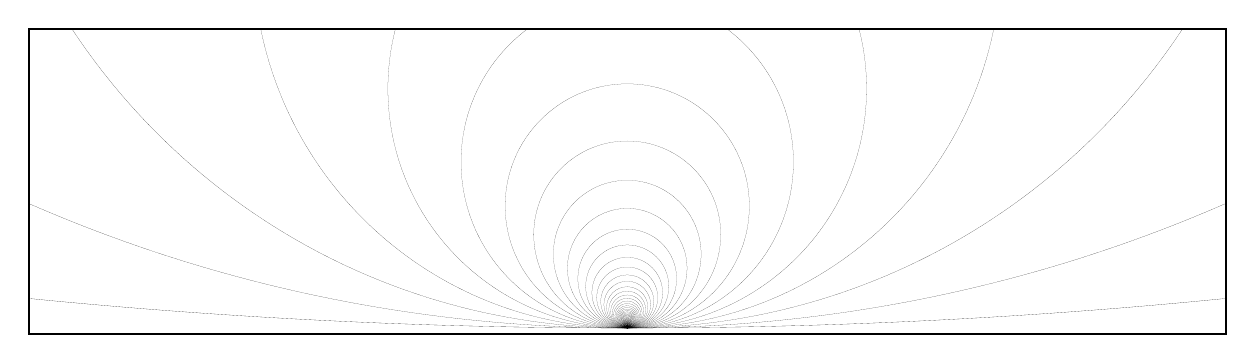
\begin{tikzpicture}[scale = 76]
	\draw[thick] (-.1,-.001) rectangle (.1,.05);
	\clip (-.1,0) rectangle (.1,.05); % remove for all circles
	\foreach \i in {1,...,100}{
		\draw[line width=0.1/\i mm] (0, 1/\i^2) circle (1/\i^2);
	}
	\end{tikzpicture}
	\caption{A closeup of the Hawaiian earring $\mathbb{H}^1$.}
\end{figure}

\begin{thm} \label{t:counterexample}
	The function $f \colon \HE \to \R$ whose value at the origin is $0$ and is $1$ everywhere else defines a compact $\LC$ sublevel set filtration that is not q-tame with respect to $\H$ if $\H_{n}(\HE)$ is not finite dimensional for some $n$.
\end{thm}

\begin{proof}
	To verify that $f$ has compact sublevel sets we notice that all sublevel sets are either the empty set, the singleton containing the origin, or $\HE$ itself, all compact Hausdorff spaces.
	
	Let us now verify that the sublevel set filtration of $f$ is $\LC$, so
	consider $x \in \HE$, $V$ a neighborhood of $x$ in $\HE$ and $t > f(x)$. We need to find a neighborhood $U \subseteq V$ of $x$ and $s \in (f(x), t)$ such that the inclusion $f_{\leq s} \cap U \to f_{\leq t} \cap V$ is homotopic to a constant map.
	
	If $x$ is the origin, we have $f(x) = 0$ and choose $s \in (0, \min\{t, 1\})$.
	Then $f_{\leq s} = \{x\}$, so with $U = V$ the inclusion $f_{\leq s} \cap U \to f_{\leq t} \cap V$ is the inclusion of $\{x\}$ into $f_{\leq t} \cap V$, which is a constant map, so the weak $\LC$ condition is trivially satisfied.
	
	For $x$ not the origin we have $f(x) = 1$ and choose $s \in (1,t)$ arbitrarily, so that $f_{\leq s} = f_{\leq t} = \HE$. 
	Note that because $x$ is not the origin, there is a unique $d$-sphere in $\HE$ that contains it.
	Clearly, we may choose $\delta > 0$ so small that $D_{\delta}(x) = \{y \in \R^{d+1} \mid \Vert x - y \Vert < \delta\} \cap \HE$ is a disk contained in this sphere and contained in $V$. 
	The disk $D_\delta(x)$ can be contracted to $\{x\}$ in $V$, so choosing $U = D_{\delta}(x)$, we obtain that the inclusion $f_{\leq s} \cap U \to f_{\leq t} \cap V$ is homotopic to the constant map with value $x$.
	
	What remains to be shown is that $f_{\leq \bullet}$ is not q-tame for $\H$.
	This follows directly from our assumption that $\H_{n}(\HE)$ is not finite dimensional for some $n$ because $f_{\leq t}$ is constant with value $\HE$ for $t \geq 1$.
\end{proof}

Both singular and \v{C}ech homology of the Hawaiian earring are infinite dimensional in some degree, so they satisfy the assumptions of \cref{t:counterexample}.
The singular case is treated in \cite{Barratt.1962}, and for \v{C}ech homology, one can use the fact that it commutes with totally ordered limits for compact Hausdorff spaces \cite[Theorems VIII.3.6.\@ and X.3.1.]{Eilenberg.1952}:
Define 
\begin{align*}
\HE_k &=
\left\{ (x_0, \dots, x_d) \in \R^{d+1} \ \middle| \ \left( x_0 - \frac{1}{k} \right)^2 + x_1^2 + \dots + x_d^2 \leq \left( \frac{1}{k} \right)^2 \right\} \\ &\cup
\bigcup_{n=1}^{k-1} \left\{ (x_0, \dots, x_d) \in \R^{d+1} \ \middle |\ \left( x_0 - \frac{1}{n} \right)^2 + x_1^2 + \dots + x_d^2 = \left( \frac{1}{n} \right)^2 \right\},
\end{align*}
i.e., the $d$-dimensional Hawaiian earring but with the $k$-th largest $d$-sphere filled.
We have $\lim_{k} \HE_{k} = \bigcap_{k} \HE_{k} = \HE$, and hence $\CH_{d}(\HE; \mathbb{F}) = \lim_{k} \CH_{d}(\HE_{k}; \mathbb{F})$, where $\CH$ denotes \v{C}ech homology.
Clearly, each $\HE_{k}$ is a CW-complex, so we can simply use cellular homology to compute
\begin{equation*}
\lim_{k}\CH_{d}(\mathbb{H}^{d}_{k}; \mathbb{F})=\lim\left(\dots\to \prod_{n=1}^2\mathbb{F}\to \prod_{n=1}^1\mathbb{F}\to \prod_{n=1}^0\mathbb{F}\right)=\prod_{n\in\mathbb{N}}\mathbb{F},
\end{equation*}
which is infinite-dimensional over $\mathbb{F}$.

\begin{cor} \label{c: counterexample}
	The function $f \colon \HE \to \R$ whose value at the origin is $0$ and is $1$ everywhere else defines a weakly $\LC$ compact sublevel set filtration that is not q-tame with respect to singular and \v{C}ech homology.
\end{cor}

The gap we have highlighted in the argument of Morse and Tompkins can be fixed by applying \cref{t:strong local connectedness implies q-tameness} because the proof given in \cite[p.464]{Morse.1939} for local connectivity of $(\Omega_g, A_g)$ actually establishes a stronger property for the sublevel set filtration of $A_g$, which we now formalize.

\begin{defi}
	The sublevel set filtration of a function $f \colon X \to \R$ is said to be \emph{strongly} $\LC$ if for any $x \in X$, any neighborhood $V$ of $x$ and any pair of indices $f(x) < s < t$ there is a neighborhood $U \subseteq V$ of $x$ such that the map $f_{\leq s} \cap U \to f_{\leq t} \cap V$ is homotopic to a constant map.
\end{defi}

Clearly, the filtration being strongly $\LC$ implies that the filtration is also strongly $\HLC$ for \v{C}ech homology with field coefficients, which is what Morse and Tompkins use.
Therefore, from \cref{t:strong local connectedness implies q-tameness} we can conclude that $(\Omega_g, A_g)$ is \mbox{q-tame} as claimed.
This implies that Morse inequalities hold, and hence so does the Morse-Tompkins' Unstable Minimal Surfaces Theorem.

We have also mentioned that Morse introduced another condition that he also called local $F$-connectivity three years earlier.
It roughly corresponds to being \emph{strongly} $\piLC$ with a certain added uniformity property.
In the original it reads:
\begin{displaycquote}[p.421-422]{Morse.1937}
	The space $M$ will be said to be locally $F$-connected for the order $n$ if corresponding to $n$, an arbitrary point $p$ on $M$, and an arbitrary positive constant $e$, there exists a positive constant $\delta$ with the following property.
	For $c \geq F(p)$ any singular $n$-sphere on $F \leq c$ (the continuous image on $F \leq c$ of an ordinary $n$-sphere) on the $\delta$-neighborhood $p_{\delta}$ of $p$ is the boundary of a singular $(n + 1)$-cell on $F \leq c + e$ and on $p_e$.
\end{displaycquote}
Morse also claims in the given reference that this condition is sufficient for q-tameness, but without providing a proof.
Whether this statement is true or not is not covered by our analysis, because the $\piLC$ and $\HLC$ conditions generally do not imply each other.
We expect the quoted claim to be true, but do not investigate it further.

\appendix

\section{Vietoris and \texorpdfstring{\v{C}}{}ech homology} \label{s:vietoris}

For greater generality, in this paper we considered \v{C}ech homology instead of the homology construction used by Morse in functional topology: metric Vietoris homology.
We now justify this choice by showing that these two constructions agree on compact metric spaces.

First, let us recall the definition of \v{C}ech homology as presented for example by \citet[Section~IX--X]{Eilenberg.1952}.
Let $X$ be a topological space and let $\Cov(X)$ be the set of all open covers of $X$ ordered by the refinement relation. 
Recall that for an open cover $\alpha \in \Cov(X)$ its \emph{nerve} $\Nrv(\alpha)$ is defined as the simplicial complex
\begin{equation*}
\Nrv(\alpha) =
\big\{ \beta \subseteq \alpha \mid \beta \text{ is finite and } \textstyle{\bigcap_{U \in \beta}} \, U \neq \emptyset \big\}.
\end{equation*}
The nerve construction defines a functor from the poset $\Cov(X)$ regarded as a category to that of simplicial complexes. 
The \emph{\v{C}ech homology with coefficients in $\F$} of $X$ is defined as
\begin{equation*}
\CH(X; \F) \ =
\lim_{\alpha \in \Cov(X)} H(\Nrv(\alpha); \F).
\end{equation*}
As an alternative to the nerve construction, for a cover $\alpha \in \Cov(X)$ one can define $\Vietoris(\alpha)$ as the simplicial complex
\begin{equation*}
\Vietoris (\alpha) = \left\{ \sigma \subseteq X \mid \sigma \text{ is finite and } \sigma \in U \text{ for some } U \in \alpha \right\},
\end{equation*}
which again yields a functor from $\Cov(X)$ to simplicial complexes.
This construction is dual to the nerve construction in the sense of Dowker's Theorem \cite{Dowker.1952}, which asserts that the two complexes $\Nrv (\alpha)$ and $\Vietoris (\alpha)$ are homotopy equivalent.
As a consequence, we have that $H (\Nrv (\alpha); \F) \cong H (\Vietoris (\alpha); \F)$.
This isomorphism is natural with respect to refinement of covers, so we get an alternative description of \v{C}ech homology as 
\begin{equation*}
\CH (X; \F) \ \cong
\lim_{\alpha \in \Cov (X)} H (\Vietoris (\alpha); \F).
\end{equation*}

If $X$ is a metric space, this is still not exactly the same as the construction of metric Vietoris homology presented in \cite{Vietoris.1927} and used by Morse, which in modern notation is the limit
\begin{equation*}
\lim_{\alpha \in \Balls(X)} H (\Vietoris (\alpha); \F),
\end{equation*}
where 
\begin{equation*}
\Balls (X) = \left\{ ( B_{\delta} (x) )_{x \in X} \mid \delta > 0 \right\}
\subseteq \Cov (X).
\end{equation*}
However, if the metric space $X$ is compact, then $\Balls (X)$ is coinitial in $\Cov (X)$, that is to say, they both define the same limit.
Thus, we have a natural isomorphism
\begin{equation*}
\CH (X; \F) \ \cong \,
\lim_{\alpha \in \Balls(X)} H (\Vietoris (\alpha); \F)
\end{equation*}
for a compact metric space $X$.
In other words, the metric Vietoris homology theory employed in Morse's setting is canonically isomorphic to the \v{C}ech homology we consider in this paper.


\section*{Acknowledgements}
This research has been supported by German Research Foundation (DFG) through the Collaborative Research Center SFB/TRR 109 \emph{Discretization in Geometry and Dynamics}, the Collaborative Research Center SFB/TRR 191 \emph{Symplectic Structures in Geometry, Algebra and Dynamics}, the Cluster of Excellence EXC-2181/1 \emph{STRUCTURES}, and the Research Training Group RTG 2229 \emph{Asymptotic Invariants and Limits of Groups and Spaces}.

A.M-M. acknowledges financial support from Innosuisse grant \mbox{32875.1 IP-ICT-1} and the hospitality of the Laboratory for Topology and Neuroscience at EPFL, where part of this work developed.

\bibliographystyle{abbrvnaturl}
\bibliography{biblio}

\end{document}